\section{Data}

The middle European electricity Market cannot be attributed to one country only. However, we focus on Germany as the four biggest Players (EoN, RWE, Vattenfal and EnBW) and the most important electricity exchange in the Region, the EEX are situated there. There are significant import capacities from Austria, Switzerland, France, the Benelux countries, the Netherlands, Denmark, Poland and the Check Republic (see \cite{Ellersdorfer2005}p. 30). Other electricity Exchanges are in Austria (EXAA), The Netherlands (APX) and in France (Powernext). Apart from energy exchanges, there are OTC Markets as well for which data are hard to get. However, Prices at the electricity exchange are generally regarded as a reliable price signal, also for the OTC Market. \cite{Holler2006} compare OTC prices and prices from the exchanges (EEX and EXAA) in Austria and Germany and conclude that both prices seem to reflect one market in the respective countries. Furthermore, they look at correlations between market prices at the different exchanges and come to the conclusion, that prices at the EEX, EXAA and Powernext are highly correlated. However, only about four Percent of the French electricity consumption is traded at the spot market and the whole French industry is heavily dominated by EDF which casts some doubt on whether there is a working electricity market in France. This is why we do not model France as a strategic part of the market which does not mean that research on that topic would not be interesting. Furthermore, the only countries where transmission lines are not congested at the moment, are Germany and Austria\footnote{An Overview of Current Cross-boarder Congestion Management Methods in Europe, www.etso-net.org} which is why we restrict our analysis to to two latter countries. 

Figure \ref{fig:ldc}

\begin{figure}[h]
\centering
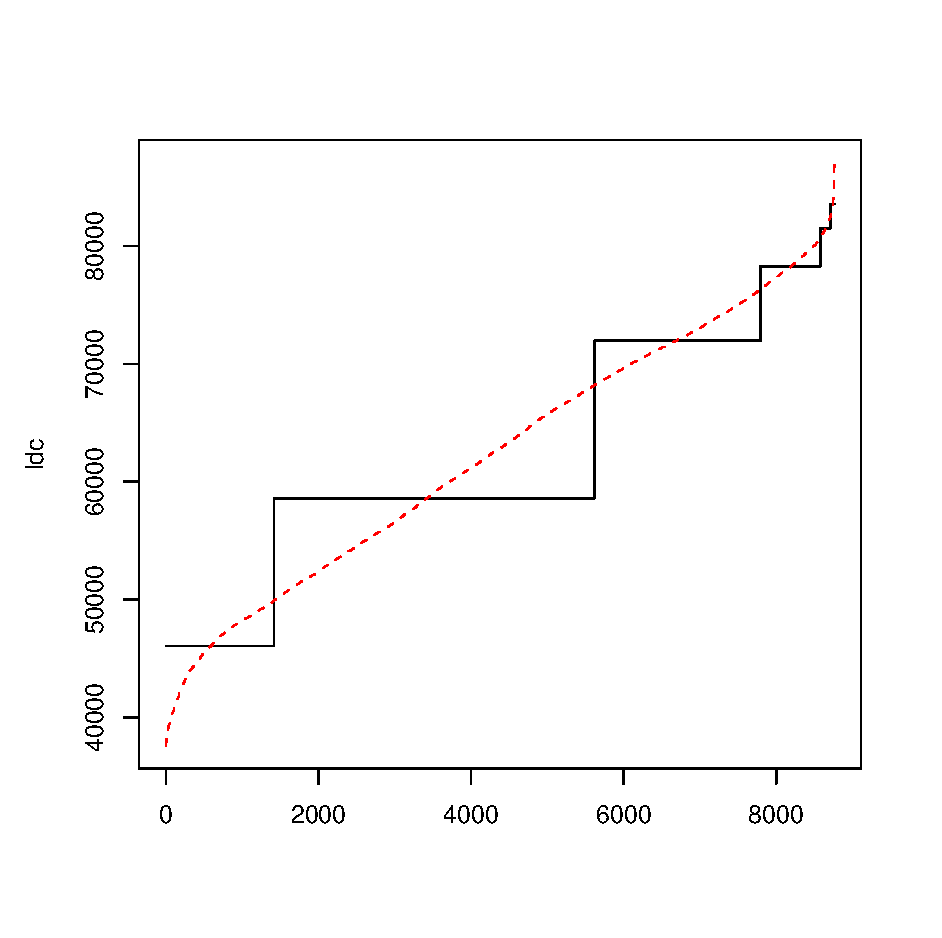
\includegraphics[width=.5\textwidth]{data/ldc}
      \label{fig:ldc}
      \caption{Load Duration Curve in MWh for Austria and Germany}
      source: 
\end{figure}


If companies prefer to use energy exchanges over the OTC market depends on the regulatory setting. How is this in Germany and Austria?

Therefore, we need data for the major players in both countries. There are no serious network congestions on the border between Austria and Germany. (for reference see Todem)

For the supply we need for every player

\begin{itemize}
\item variable and fixed costs,
\item structure of the plant park.
\end{itemize}

Parameters for the demand curve are obtained from

\begin{itemize}
\item load duration curve
\item how parameters for demand functions from load duration curve
\end{itemize}

Show that Austrian players are fringe? 

Long term structure of plant parks.

How does the resulting plant park structure look like, if firms actually play two-stage open or closed-looped games and other possible market structures (perfect competition, Betrand). 

How could the current market structures look like one long term step ahead (in ten years from now, one investment cycle).

Welfare implications from different market structures.

Implications of capacity markets.

